\begin{abcliste}
\abc Hutmacher fährt die Strecke $N\,\ell$ in der Zeit $t_\mathrm{H} = \tHhO\ \tHmO\ \tHsO = \tH$:
\begin{align}
 v_\mathrm{H} &= \vHF = \frac{\NR\cdot\lR}{\tH} \\
   &= \vH \approx \result{\vHkP{0}{3}}
\end{align}

\abc Hutmacher überrundet Jacqueline jedes Mal, wenn sein Vorsprung um eine weitere Runde $\ell$ gewachsen ist. Der Vorsprung wächst mit der Differenz der Geschwindigkeiten,
\begin{align}
 \Delta v &= \dvF = \vH-\vJ = \dv \approx \dvkP{0}{2}
\end{align}

\emph{Graphisch:} Man zeichnet den Vorsprung $\Delta s = \Delta v\cdot t$ gegen die Zeit und dazu die Linien $\Delta s = \ell$, $2\ell$, $3\ell$. Die Schnittpunkte geben die Zeitpunkte der Überrundungen; die Gerade endet bei $t_\mathrm{H}$, wenn Hutmacher im Ziel ist.

\begin{center}
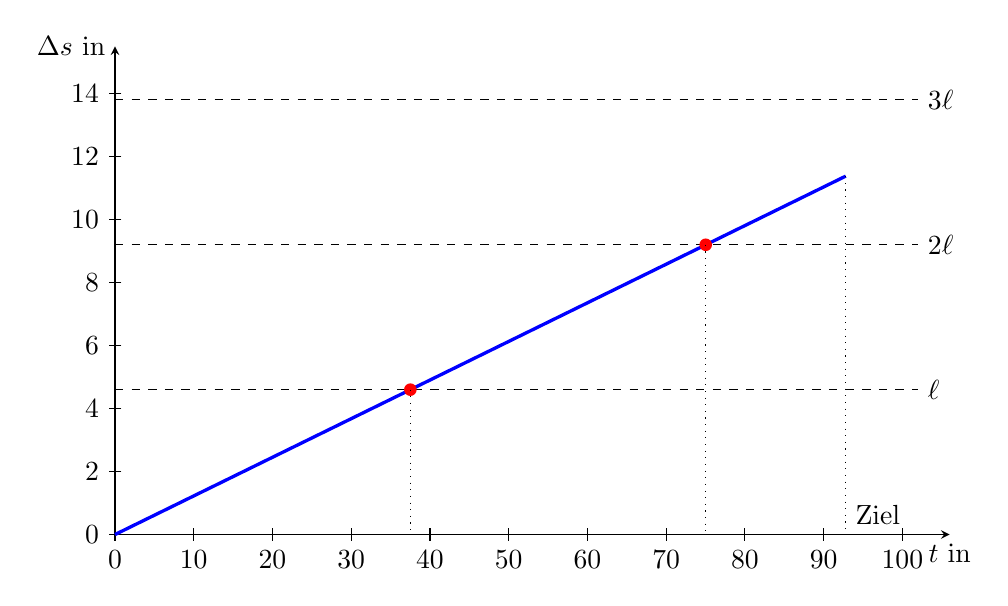
\begin{tikzpicture}[>=stealth]
 \draw[->] (0,0) -- (10.6,0) node[below] {$t$ in \si{\minute}};
 \draw[->] (0,0) -- (0,6.2) node[left] {$\Delta s$ in \si{\km}};
 \foreach \x in {0,10,...,100} \draw (\x/10,0.08) -- (\x/10,-0.08) node[below] {\x};
 \foreach \y in {0,2,...,14} \draw (0.08,\y*0.4) -- (-0.08,\y*0.4) node[left] {\y};
 \foreach \x/\lab in {1/\ell, 2/2\ell, 3/3\ell} \draw[dashed] (0,\x*1.84) -- (10.2,\x*1.84) node[right] {$\lab$};
 \draw[blue, very thick] (0,0) -- (9.281,4.552);
 \draw[dotted] (9.281,4.552) -- (9.281,0) node[above right] {Ziel};
 \fill[red] (3.751,1.84) circle (0.08);
 \fill[red] (7.502,3.68) circle (0.08);
 \draw[dotted] (3.751,1.84) -- (3.751,0);
 \draw[dotted] (7.502,3.68) -- (7.502,0);
\end{tikzpicture}
\end{center}
Die Gerade schneidet die Linien $\ell$ und $2\ell$ (nach $t_1 \approx \tUmP{0}{2}$ und nach $2\,t_1$), aber nicht mehr $3\ell$: Es gibt zwei Überrundungen.

\emph{Algebraisch:} Die erste Überrundung erfolgt nach
\begin{align}
 t_1 &= \tUF = \frac{\lR}{\dv} = \tU \approx \tUmP{0}{2}
\end{align}
Bis dahin hat Hutmacher
\begin{align}
 n_1 &= \frac{v_\mathrm{H}\,t_1}{\ell} = \nUF = \frac{\vH}{\dv} = \nUQ
\end{align}
Runden zurückgelegt. Er überrundet Jacqueline also erstmals in seiner $\result{\rUI.}$~Runde, ein zweites Mal nach $n_2 = 2\,n_1 = \nZQ$ Runden, also in der \rZI.~Runde. Bis zum Ziel wächst der Vorsprung auf
\begin{align}
 k &= \kUF = \frac{\left(\dv\right)\cdot\tH}{\lR} = \kUQ
\end{align}
Runden. Hutmacher überrundet Jacqueline also insgesamt $\result{\kGI}$-mal.
\end{abcliste}
